\documentclass[a4paper, french, 8pt]{report}
\title{NF92 TP \LaTeX}
\author{Prénom NOM (Compte NF92)}
\date{Last edition : \today}
\usepackage[french]{babel}
\usepackage[utf8]{inputenc}
\usepackage[T1]{fontenc}
\usepackage{graphicx}
\usepackage{geometry} \geometry{hmargin=3cm,vmargin=2.5cm}
\usepackage{fancyhdr}
\usepackage{amsmath}

%%%% Début de Macro définissant un débordement du texte dans la marge (dans le sujet) %%%%
\newenvironment{changemargin}{\begin{list}{}{
\setlength{\rightmargin}{-1.5cm}
\setlength{\leftmargin}{0.5cm}
}\item }{\end{list}}
%%%% Fin de Macro définissant un débordement du texte dans la marge %%%%

\begin{document}

\maketitle
\listoffigures
\listoftables

\begin{abstract}

\indent Dans ce livrable en LaTex, nous étions face à l'environnement LaTex et ses différentes possibilités. Nous devions donc à l'aide d'internet et des connaissances apportées en cours, reproduire un livrable modèle le plus justement possible. Un ensemble de notions LaTex ont été explorées dans les différentes parties du livrable. Le chapitre \ref{chapitre1} était une initiation à de nombreuses notions plutôt simples telles que la formation des caractères spéciaux qui nous mettait au défis de réussir à écrire les commandes telles quelles sans que latex les exécute et de les referencer dans un texte ( voir dans la section \ref{section1} le tableau \ref{tableau1}) ou encore le placement d'image à la suite d'un texte (avec un angle de 20\degre) et en faire référence dans un texte comme dans la section \ref{section2} avec les images \ref{logo_fedora_droit} et \ref{logo_fedora_incline}.

\medskip
\indent Ensuite le chapitre \ref{chapitre2} traitait de la possibilité mathématique apportée par le latex. Dans la section \ref{section3} nous avons réalisé une matrice complexe puis une equation ( voir equation \ref{equation1}) que nous avons referencée dans le texte du dessous. Nous avons aussi eu la possibilité de rajouter une bibliographie à l'aide de nombreuses commandes, puis de referencer certains auteurs dans les textes.

\medskip
\indent Par la suite, dans la section \ref{section4}, nous avons exploré la possibilité d'ajouter une figure mathématique ( figure \ref{graph}) et de la référencer dans le texte. 

\medskip
\indent Pour finir la section \ref{section5}, nous a confronté au fait de devoir recopier le plus parfaitement possible un texte en anglais comprenant plusieurs equations (équations \ref{equation2} et \ref{equation3}) ainsi qu'un tableau (tableau \ref{tableau2}). Des références à la bibliographie était aussi demandées.   
\end{abstract}

\chapter{Début}
\label{chapitre1}

\section{Caractères spéciaux}
\label{section1}
Ajoutez une section qui comporte un tableau de deux colonnes. La colonne de gauche contiendra le résultat affiché par \LaTeX après compilation, la colonne de droite contiendra la commande \LaTeX à utiliser pour pouvoir l'obtenir. \textbf{Attention}, il faudra trouver le moyen d'empêcher \LaTeX d'utiliser cette commande, à vous de trouver. Ajoutez une légende et trouvez comment y ajouter un label pour y faire plus tard référence (i.e. \textit{Cross-Reference}). \medskip

Ce tableau traitera des caractères \$ \& \% \# \{ \} \_ etc. Le début de cette table est dans la Table 1.

    \begin{table}[h]
        \centering
        \begin{tabular}{|c|c|}
             \hline
             Caractères spéciaux & Commandes \\
             \hline
             \hline
             \$ & \textbackslash\$ \\ 
             \hline
             \& & \textbackslash\& \\
             \hline
             \% & \textbackslash\% \\
             \hline
             \# & \textbackslash\# \\
             \hline
             \{ & \textbackslash\{ \\
             \hline
             \} & \textbackslash\} \\
             \hline
             \_ & \textbackslash\_ \\
             \hline
             \ldots & \textbackslash ldots \\
             \hline
        \end{tabular}
        \caption{Début de la table des caractères spéciaux}
        \label{tableau1}
    \end{table}
    
Les caractères spéciaux ne sont donc pas simplement insérés comme des lettres, mais bien avec des commandes propres à \LaTeX . Cependant, ces commandes sont la plupart du temps simples à mémoriser, car, comme le montre la Table \ref{tableau1}, elles allient en général simplement le backslash (\textbackslash) au caractère lui même.

\newpage
\section{Images}
\label{section2}
\begin{figure}[!h]
    \centering
    
\includegraphics[scale=0.3]{fedora.eps}
    \caption{Un logo fedora core}
    \label{logo_fedora_droit}
\end{figure}

\begin{figure}[!h]
    \centering
    
\includegraphics[scale=0.3, angle=20]{fedora.eps}
    \caption{Un logo fedora core avec un angle de 20\degre}
    \label{logo_fedora_incline}
\end{figure}


 Pour inclure une image dans le doucment \LaTeX, à la manière des images \ref{logo_fedora_droit} et \ref{logo_fedora_incline}, il suffit d'entrer la fonction \textbackslash includegraphics $\{$nomDeVotreImage.format$\}$. Pour l'incliner (comme l'image \ref{logo_fedora_incline}), il suffit simplement d'ajouter le paramètre [angle=valeurDeLAngle] après le \textbackslash includegraphics.

\chapter{Travail réalisé}
\label{chapitre2}

\section{Référence aux formules}
\label{section3}
Le déterminant d'une matrice $3 \times 3$ est :

\[
\begin{vmatrix} A \end{vmatrix} = 
\begin{vmatrix}
~ a & b & c\\
~ d & e & f\\
~ g & h & i
\end{vmatrix}  = 
a \times 
\begin{vmatrix}
~ e & f\\
~ h & i\\
\end{vmatrix}
- b \times 
\begin{vmatrix}
~ d & f\\
~ g & i\\
\end{vmatrix}
- c \times 
\begin{vmatrix}
~ d & e\\
~ g & h\\
\end{vmatrix}
\]

Soit :
\begin{equation}
  \Delta (A) = aei + bfg + cdh - ceg - bdi - afh 
  \label{equation1}
  \tag{1}
\end{equation}
Si $ \Delta (A) = \begin{vmatrix} A \end{vmatrix} = det(A) = 0 $, calculé avec l'équation \ref{equation1}, alors il n'y a pas une unique solution au système matriciel. \\
Ce qui n'a strictement rien à voir avec le travail présenté dans les articles \cite{burke1997automated, springerlink:10.1007/s10479-011-0997-x}.

\section{Exemples de graphs}
\label{section4}

\begin{figure}[!h]
    \centering
    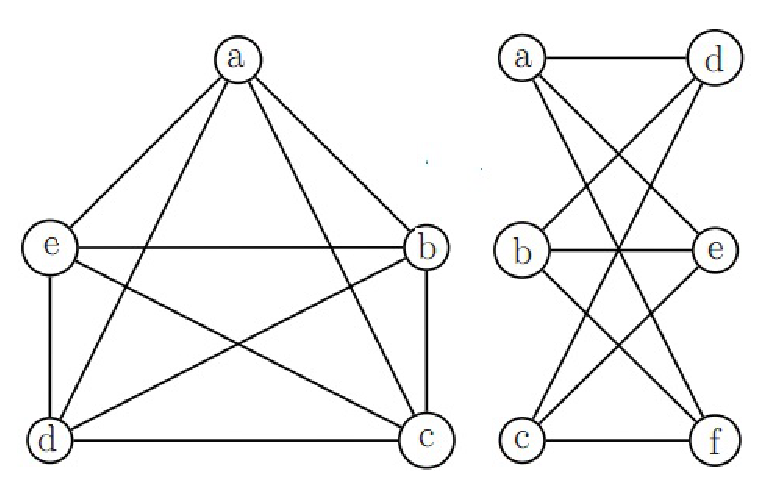
\includegraphics[scale=0.5]{K5_K3_3_Graph.eps}
    \caption{A gauche la clique K5, à droite K3 3 un graphe biparti complet}
    \label{graph}
\end{figure}

Considérons la Figure \ref{graph} : cinq couleurs sont nécessaires pour colorier le graphe K5, tandis que deux suffisent pour K3\_3. Cependant un graphe est planaire s’il ne contient parmi ses mineurs aucun des graphes de la Figure \ref{graph}.

\section{The Original Model}
\label{section5}

\begin{changemargin}We address the examination timetabling problem proposed in the second International Timetabling\end{changemargin}Competition (ITC2007). The reader should refer to \cite{burke1997automated} for a detailed overview of examination time tabling.

We present in the sequel the original model proposed by \cite{springerlink:10.1007/s10479-011-0997-x}. As stated by the authors, the aim was to give a clear model. We invite the reader to refer to the original paper for comprehensive details.

In \cite{springerlink:10.1007/s10479-011-0997-x}, the authors introduced the conflict graph $G(E, A_C )$, where $E$ is the set of exams and an edge $[i, j] \in A_C$ if there is at least one student enrolled in exams $i$ and $j$. An edge $[i, j]$ is weighted by $w^C_{ij}$ , the number of students taking the two exams. The core problem is to find a graph coloring. Note that \cite{sabar2012graph} derived a hyper-heuristic based on graph coloring constructive ordering heuristics to select exams to be scheduled. $P$, $R$ and $S$ denote the sets of periods, rooms and students respectively. For the sake of compactness, the objective function and the hard constraints of the model have been rewritten as:

Minimize:

\begin{equation}
	C^{2D}
	\label{equation2}
	\tag{2}
\end{equation}
Subject to :
\begin{equation}
	\forall i \in E ~ \sum_{p \in P} \sum_{r \in R} X_{ipr}^{PR} \le 1
	\label{equation3}
	\tag{3}
\end{equation}

\begin{equation}
	\forall p\in P ~ \forall r \in R ~ \sum_{i \in E} s_{i}^{E} C_{ipr}^{PR} \le s_{r}^{R}
    \label{equation4}
	\tag{4}
\end{equation}

\begin{equation}
	\forall i \in E ~ \forall p \in P ~ \sum_{j \in N (i)} X_{jp}^{P} + a_{ip} X_{ip}^{PR} \le a_{ip}
	\label{equation5}
	\tag{5}
\end{equation}

\begin{equation}
	C^{2D} = w^{2D} ~ \sum_{[i,j] \in A_C} w_{ij}^{C} C_{ij}^{2D}
	\label{equation6}
	\tag{6}
\end{equation}

\begin{equation}
    \left.
    \begin{array}{r}
  
        \forall [i,j] \in A_C ~ \forall p,q \in P ~ with ~ |p-q| = 1 \\
        with ~ y_{pq} = 1 X_{ip}^{P} + X_{jq}^{P} \le 1 + C_{ij}^{2D}
        
    \end{array}
    \right \}
    \label{equation7}
    \tag{7}
\end{equation}

\indent Equations (\ref{equation3})  ensure that all the exams are allocated once to a unique period and a unique
 room. The room capacities are always respected using Equations (\ref{equation4}) in which $s_i^E$ and $s_r^R$
 denote the number of students sitting exam \textit{i} and the seating capacity of room \textit{r} respectively.\\
 \indent Equations (\ref{equation5}) enforce the conflict constraints: at any period, any student will be sitting
 at most one exam.\\
 \indent The boolean variables used to count the number of \textbf{Two In Day} penalties are $C_{ij}^{2D}$, 
 $C_{ij}^{2D}$=1 iff two exams are allocated in the same days but not back to back. The integer
 variable  $C^{2D}$ is used to compute the objective fonction (see Equation (\ref{equation2})). \\
 \indent The \textbf{Two In a Day} term  $C^{2D}$ is set by Equations (\ref{equation6}) and (\ref{equation7}), in which the boolean 
 parameter $y_{pq}$=1 periods \textit{p} and \textit{q} are on the same day.

\begin{table}[h]
 \begin{center}
    \caption{Characteristics of the Yeditepe datasets}
    \label{tableau2}
    \begin{tabular}{r|r r r r||r r||r}
       & \textit{$n^E$} & \textit{$n^S$} & \textit{$n^P$} & \textit{$n^R$} &\textit{$w_{A_C}$} & \textit{$n_{w_{A_C}}$} & $t_{\alpha _{ip}}$\\ 
        \hline
    yue20011 & 126 & 569 & 18 & 2 & 14 & 78 & 1\\
    yue20012 & 141 & 581 & 18 & 2 & 17 & 8 & 0\\
    yue20023 & 38 & 224 & 6 & 1 & 6 & 4 & 1\\
 \end{tabular}
 \end{center}
 \ref{tableau2}
\end{table}
The Characteristics of the Yeditepe datasets used for our tests are displayed in Table 


\bibliographystyle{plain}
%\bibliographystyle{abbr}
%\bibliographystyle{alpha}
\bibliography{biblio}
\end{document}